\documentclass[12pt]{article}
\usepackage[margin = 1in]{geometry}
\usepackage{setspace}
\usepackage{amsmath}
\usepackage{amssymb}
\usepackage{amsthm}
\usepackage{graphicx}
\usepackage{subfig}
\usepackage{enumitem}
\usepackage{url}
\usepackage[parfill]{parskip}
\usepackage{listings}
\newcommand{\skipline}{\vspace{\baselineskip}}
\newcommand{\spacer}{\noalign{\medskip}}
\newenvironment{problem}[1]{\textbf{Problem #1: }}{\newpage}
\newenvironment{Section}[1]{}{\newpage}

% Options for packages loaded elsewhere
\PassOptionsToPackage{unicode}{hyperref}
\PassOptionsToPackage{hyphens}{url}
\usepackage{lmodern}
\usepackage{amssymb,amsmath}
\usepackage{ifxetex,ifluatex}
\ifnum 0\ifxetex 1\fi\ifluatex 1\fi=0 % if pdftex
\usepackage[T1]{fontenc}
\usepackage[utf8]{inputenc}
\usepackage{textcomp} % provide euro and other symbols
\else % if luatex or xetex
\usepackage{unicode-math}
\defaultfontfeatures{Scale=MatchLowercase}
\defaultfontfeatures[\rmfamily]{Ligatures=TeX,Scale=1}
\fi
% Use upquote if available, for straight quotes in verbatim environments
\IfFileExists{upquote.sty}{\usepackage{upquote}}{}
\IfFileExists{microtype.sty}{% use microtype if available
	\usepackage[]{microtype}
	\UseMicrotypeSet[protrusion]{basicmath} % disable protrusion for tt fonts
}{}
\makeatletter
\@ifundefined{KOMAClassName}{% if non-KOMA class
	\IfFileExists{parskip.sty}{%
		\usepackage{parskip}
	}{% else
		\setlength{\parindent}{0pt}
		\setlength{\parskip}{6pt plus 2pt minus 1pt}}
}{% if KOMA class
	\KOMAoptions{parskip=half}}
\makeatother
\usepackage{xcolor}
\IfFileExists{xurl.sty}{\usepackage{xurl}}{} % add URL line breaks if available
\IfFileExists{bookmark.sty}{\usepackage{bookmark}}{\usepackage{hyperref}}
\hypersetup{
	pdftitle={Project},
	pdfauthor={Stephen Giang},
	hidelinks,
	pdfcreator={LaTeX via pandoc}}
\urlstyle{same} % disable monospaced font for URLs
\usepackage[margin=1in]{geometry}
\usepackage{color}
\usepackage{fancyvrb}
\newcommand{\VerbBar}{|}
\newcommand{\VERB}{\Verb[commandchars=\\\{\}]}
\DefineVerbatimEnvironment{Highlighting}{Verbatim}{commandchars=\\\{\}}
% Add ',fontsize=\small' for more characters per line
\usepackage{framed}
\definecolor{shadecolor}{RGB}{248,248,248}
\newenvironment{Shaded}{\begin{snugshade}}{\end{snugshade}}
\newcommand{\AlertTok}[1]{\textcolor[rgb]{0.94,0.16,0.16}{#1}}
\newcommand{\AnnotationTok}[1]{\textcolor[rgb]{0.56,0.35,0.01}{\textbf{\textit{#1}}}}
\newcommand{\AttributeTok}[1]{\textcolor[rgb]{0.77,0.63,0.00}{#1}}
\newcommand{\BaseNTok}[1]{\textcolor[rgb]{0.00,0.00,0.81}{#1}}
\newcommand{\BuiltInTok}[1]{#1}
\newcommand{\CharTok}[1]{\textcolor[rgb]{0.31,0.60,0.02}{#1}}
\newcommand{\CommentTok}[1]{\textcolor[rgb]{0.56,0.35,0.01}{\textit{#1}}}
\newcommand{\CommentVarTok}[1]{\textcolor[rgb]{0.56,0.35,0.01}{\textbf{\textit{#1}}}}
\newcommand{\ConstantTok}[1]{\textcolor[rgb]{0.00,0.00,0.00}{#1}}
\newcommand{\ControlFlowTok}[1]{\textcolor[rgb]{0.13,0.29,0.53}{\textbf{#1}}}
\newcommand{\DataTypeTok}[1]{\textcolor[rgb]{0.13,0.29,0.53}{#1}}
\newcommand{\DecValTok}[1]{\textcolor[rgb]{0.00,0.00,0.81}{#1}}
\newcommand{\DocumentationTok}[1]{\textcolor[rgb]{0.56,0.35,0.01}{\textbf{\textit{#1}}}}
\newcommand{\ErrorTok}[1]{\textcolor[rgb]{0.64,0.00,0.00}{\textbf{#1}}}
\newcommand{\ExtensionTok}[1]{#1}
\newcommand{\FloatTok}[1]{\textcolor[rgb]{0.00,0.00,0.81}{#1}}
\newcommand{\FunctionTok}[1]{\textcolor[rgb]{0.00,0.00,0.00}{#1}}
\newcommand{\ImportTok}[1]{#1}
\newcommand{\InformationTok}[1]{\textcolor[rgb]{0.56,0.35,0.01}{\textbf{\textit{#1}}}}
\newcommand{\KeywordTok}[1]{\textcolor[rgb]{0.13,0.29,0.53}{\textbf{#1}}}
\newcommand{\NormalTok}[1]{#1}
\newcommand{\OperatorTok}[1]{\textcolor[rgb]{0.81,0.36,0.00}{\textbf{#1}}}
\newcommand{\OtherTok}[1]{\textcolor[rgb]{0.56,0.35,0.01}{#1}}
\newcommand{\PreprocessorTok}[1]{\textcolor[rgb]{0.56,0.35,0.01}{\textit{#1}}}
\newcommand{\RegionMarkerTok}[1]{#1}
\newcommand{\SpecialCharTok}[1]{\textcolor[rgb]{0.00,0.00,0.00}{#1}}
\newcommand{\SpecialStringTok}[1]{\textcolor[rgb]{0.31,0.60,0.02}{#1}}
\newcommand{\StringTok}[1]{\textcolor[rgb]{0.31,0.60,0.02}{#1}}
\newcommand{\VariableTok}[1]{\textcolor[rgb]{0.00,0.00,0.00}{#1}}
\newcommand{\VerbatimStringTok}[1]{\textcolor[rgb]{0.31,0.60,0.02}{#1}}
\newcommand{\WarningTok}[1]{\textcolor[rgb]{0.56,0.35,0.01}{\textbf{\textit{#1}}}}
\usepackage{graphicx,grffile}
\makeatletter
\def\maxwidth{\ifdim\Gin@nat@width>\linewidth\linewidth\else\Gin@nat@width\fi}
\def\maxheight{\ifdim\Gin@nat@height>\textheight\textheight\else\Gin@nat@height\fi}
\makeatother
% Scale images if necessary, so that they will not overflow the page
% margins by default, and it is still possible to overwrite the defaults
% using explicit options in \includegraphics[width, height, ...]{}
\setkeys{Gin}{width=\maxwidth,height=\maxheight,keepaspectratio}
% Set default figure placement to htbp
\makeatletter
\def\fps@figure{htbp}
\makeatother
\setlength{\emergencystretch}{3em} % prevent overfull lines
\providecommand{\tightlist}{%
	\setlength{\itemsep}{0pt}\setlength{\parskip}{0pt}}
\setcounter{secnumdepth}{-\maxdimen} % remove section numbering


\doublespacing
\begin{document}
	
	\begin{Section}{Cover Page}
		\begin{center}
			\huge 
			\textbf{The Journey to Home Ownership \\
			Show Me the Numbers \\}
			\skipline
		\end{center}
		\begin{figure}[h!]
			\centering
			\includegraphics[width = \linewidth, height = 9cm]{Figures/CoverPhoto.jpg}
		\end{figure}
		\begin{center}
			\large
			Presented and Created for: \\
			\textbf{SDSUSS-SCorp Financial Services}
		\end{center}
		\skipline
		\begin{center}
			\large
			Presented and Created by: \\
			\textbf{A+ Mortgage Market Mathematicians} \\
			Stephen Giang $\cdot$ REDID: 823184070 \\
			2718 Euler Street, E City, CA 92802 \\
			(271) 828 1828 $\cdot$ StephenGiang@ApMMM.com
		\end{center}
	\end{Section}

	\begin{Section}{Executive Summary}
		\textbf{\Huge Executive Summary}
		\\ \\
		\textbf{\large Overview}
		\\ \\
		This report covers the entire process of choosing the right loan and understanding how each loan is determined.  It will contains numbers about Credit Scores, Income, Down Payment, and more. It shows how variation in these parameters will affect the interest rates, the principle allowed to borrow, and the term length.  This report is to inform clients and future home buyers the pre-approval process of buying a home and making sure the clients are informed about every step.
		\\ \\
		\textbf{\large Goal}
		\\ \\
		Our Goal at A+ Mortgage Market Mathematicians is to create a relationship with SDSUSS-SCorp Financial Services.  This report will make the home ownership journey so much easier for clients, which will lead to amazing referrals and thus a larger clientele for your company.  
		\\ \\
		\textbf{\large Conclusions}
		\\ \\
		We were able to conclude from our findings, the different scenarios that which the average resident in San Diego may need to go through when considering opening a mortgage loan.      
	\end{Section}

	\begin{Section}{Introduction}
		\textbf{\Huge Introduction}
		\\ \\
		Many soon to be first time home owner come to financial institutions like yours very confused on what exactly they can afford, and what kind of options that are available to them.  When getting preapproved for a mortgage loan, information such as a credit history, income, and current assets, play a very big role in what kind of loans are available.  From this information, we can very roughly determine the interest rate, loan amount, and term length, the client can get preapproved for.  
		\\ \\
		For general purposes, we will roughly estimate the interest rate based off current average mortgage rates and the clients' credit score.  The average mortgage rate in San Diego is currently about 3\%.  We can use a range of values from 2.5\% - 3.5\% to represent the different interest rates based off different credit scores.  To begin a mortgage loan, clients should have a credit score ranging between 680 and 800.  From these ranges, we can determine that the lower the credit score, the higher the interest rate and vice versa.
		\\ 
		We can roughly choose a interest rate from the following:
		\begin{figure}[h!]
			\centering
			\begin{tabular}{|c|c|c|c|c|c|c|c|c|c|}
				\hline
				Interest Rate & 2.5\% & 2.625\% & 2.75\% & 2.875\% & 3.0\% & 3.125\% & 3.25\% & 3.375\% & 3.5\% \\
				\hline
				Credit Score & 800 & 785 & 770 & 755 & 740 & 725 & 710 & 695 & 680  \\
				\hline
			\end{tabular}
		\end{figure}
		\\ \\
		After choosing the interest rate, we can take the clients' income and amount for a down payment to determine the monthly payment.  The monthly payment should be less than 30\%  the clients' monthly income.  
	\end{Section}

	\begin{Section}{Data}
		\textbf{\Huge Data and Methods}
		\\ \\
		Notice we can model a simple fixed year term plan with the following: 
		\begin{align*}
			P_0 &= P \\
			P_1 &= P_0(1 + r) - x = P(1 + r) - x \\
			P_2 &= P_1(1 + r) - x = P(1 + r)^2 - x(1 + r) - x \\
			P_3 &= P_2(1 + r) - x = P(1 + r)^3 - x(1 + r)^2 - x(1 + r) - x
		\end{align*}
		with $P_i$ and $i \in \{0,1,2,3\}$ being the principle left after $i$ months, $r$ being the monthly interest rate, or the annual interest rate divided over 12 months, and $x$ being the monthly payment.
		\\ \\
		We can see from here, for some month, $k$, a loan with an initial principle, $P$, and an annual interest rate, $n$, we get the following:
		\begin{align*}
			P_{k} &= P\left(1 + \frac{n}{12}\right)^{k} - x\left[\left(1 + \frac{n}{12}\right)^{k - 1} + \left(1 + \frac{n}{12}\right)^{k - 2} + \cdots + \left(1 + \frac{n}{12}\right) + 1\right] \\
			&= P\left(1 + \frac{n}{12}\right)^{k} - x\left[\frac{\left(1 - \left(1 + \frac{n}{12}\right)^{k}\right)}{\left(1 - \left(1 + \frac{n}{12}\right) \right)}\right]
		\end{align*}
		From this we can see for a $q$ year term loan, we get that 
		\[0 = P\left(1 + \frac{n}{12}\right)^{12q} - x\left[\frac{\left(1 - \left(1 + \frac{n}{12}\right)^{12q}\right)}{\left(1 - \left(1 + \frac{n}{12}\right) \right)}\right]\]
		Using some simple algebra, we get the monthly payment:
		\[x = \frac{P\left(1 + \frac{n}{12}\right)^{12q}\left(1 - \left(1 + \frac{n}{12}\right) \right)}{\left(1 - \left(1 + \frac{n}{12}\right)^{12q}\right)}\]
		\newpage
		Because the monthly payment has to be less than 30\% of the clients' gross monthly income, we can see the following, for the clients' yearly salary, $S$:
		\[x = \frac{P\left(1 + \frac{n}{12}\right)^{12q}\left(1 - \left(1 + \frac{n}{12}\right) \right)}{\left(1 - \left(1 + \frac{n}{12}\right)^{12q}\right)} \leq \frac{.30S}{12}\]
		From this we get that the principle the client can afford will be:
		\[P \leq \frac{S\left(1 - \left(1 + \frac{n}{12}\right)^{12q}\right)}{40\left(1 + \frac{n}{12}\right)^{12q}\left(1 - \left(1 + \frac{n}{12}\right) \right)}\]
		Using this information, the client can then look for a home with a value of:
		\[H \leq \frac{S\left(1 - \left(1 + \frac{n}{12}\right)^{12q}\right)}{40\left(1 + \frac{n}{12}\right)^{12q}\left(1 - \left(1 + \frac{n}{12}\right) \right)} + D\]
		Where $H$ is the home value, and $D$ is the amount of money the client has for a down payment.
	\end{Section}

	\begin{Section}{Example A}
		\textbf{\Huge Example A}
		\\ \\
		Let there be a Client A with a credit score of 740, an annual salary of \$100,000, and looking for a 30 year term loan.  This client will represent the "average" mortgage loan in San Diego, as the average home in San Diego is \$750,000 and the average mortgage rate is 3.00\%
		\\ \\
		With a credit score of 740, we can estimate the annual interest rate to be 3.00\% and with the given salary, term length, and interest rate, Client A can be pre-approved for a max loan of \$592,973.50.  For simplicity reasons, we can round this to \$600,000.  If Client A puts a 20\% down payment, Client A would be in the market for a \$750,000 home; this is the average home value in San Diego.  With the following conditions, Client A will be paying \$2,529.62 a month on his mortgage.  By the end of the mortgage, Client A will have paid in a total of \$910,664.71 for a \$600,000 loan.  This means, the client would have paid a total of \$310,664.71 worth of interest.  This is 51.78\% the original loan in just interest.  It takes 13 years and 5 months to have paid off more principle than interest.  On a month to month aspect, it takes 7 years for the monthly payment to pay more principle than interest.
		\\ \\
		If Client A had a credit score of 785, he or she would have an annual interest rate of 2.625\%.  This would change the total interest paid to \$267,565.15.  This is a saving of \$43,099.57.  If Client A could save up some money from his or her own job as well, the client would be able to put another down payment on another property.  This would lead to a cycle of real estate and continous business for SDSUSS-SCorp Financial Services.
		\newpage 
\begin{singlespace}
\begin{Shaded}
\begin{Highlighting}[]
\CommentTok{# Functions}

\NormalTok{MonthlyPayment =}\StringTok{ }\ControlFlowTok{function}\NormalTok{(P, AIR, Term) \{}
\NormalTok{  r =}\StringTok{ }\NormalTok{AIR }\OperatorTok{/}\StringTok{ }\NormalTok{(}\DecValTok{100} \OperatorTok{*}\StringTok{ }\DecValTok{12}\NormalTok{)}
\NormalTok{  k =}\StringTok{ }\NormalTok{Term }\OperatorTok{*}\StringTok{ }\DecValTok{12}
\NormalTok{  x =}\StringTok{ }\NormalTok{(P }\OperatorTok{*}\StringTok{ }\NormalTok{(}\DecValTok{1} \OperatorTok{+}\StringTok{ }\NormalTok{r)}\OperatorTok{^}\NormalTok{k) }\OperatorTok{/}\StringTok{ }\NormalTok{( (}\DecValTok{1} \OperatorTok{-}\StringTok{ }\NormalTok{(}\DecValTok{1} \OperatorTok{+}\StringTok{ }\NormalTok{r)}\OperatorTok{^}\NormalTok{k) }\OperatorTok{/}\StringTok{ }\NormalTok{(}\DecValTok{1} \OperatorTok{-}\StringTok{ }\NormalTok{(}\DecValTok{1} \OperatorTok{+}\StringTok{ }\NormalTok{r)) )}

  \KeywordTok{return}\NormalTok{(x)}
\NormalTok{\}}

\NormalTok{PlotInfo =}\StringTok{ }\ControlFlowTok{function}\NormalTok{(P, AIR, Term) \{}
\NormalTok{  Principle =}\StringTok{ }\NormalTok{P}
\NormalTok{  r =}\StringTok{ }\NormalTok{AIR }\OperatorTok{/}\StringTok{ }\NormalTok{(}\DecValTok{100} \OperatorTok{*}\StringTok{ }\DecValTok{12}\NormalTok{)}
\NormalTok{  k =}\StringTok{ }\NormalTok{Term }\OperatorTok{*}\StringTok{ }\DecValTok{12}
\NormalTok{  x =}\StringTok{ }\KeywordTok{MonthlyPayment}\NormalTok{(P, AIR, Term)}

\NormalTok{  P =}\StringTok{ }\KeywordTok{matrix}\NormalTok{(}\DecValTok{0}\NormalTok{, }\DataTypeTok{nrow =}\NormalTok{ k }\OperatorTok{+}\StringTok{ }\DecValTok{1}\NormalTok{)}
\NormalTok{  i =}\StringTok{ }\DecValTok{1}
\NormalTok{  P[i] =}\StringTok{ }\NormalTok{Principle}
\NormalTok{  MonthPPaid =}\StringTok{ }\DecValTok{0}
\NormalTok{  AccPPaid =}\StringTok{ }\DecValTok{0}
\NormalTok{  Interest =}\StringTok{ }\DecValTok{0}
\NormalTok{  AccInterest =}\StringTok{ }\DecValTok{0}

\NormalTok{  table =}\StringTok{ }\KeywordTok{matrix}\NormalTok{( }\KeywordTok{c}\NormalTok{( (i }\OperatorTok{-}\StringTok{ }\DecValTok{1}\NormalTok{), P[i], MonthPPaid, AccPPaid, Interest,}
\NormalTok{                     AccInterest), }\DataTypeTok{nrow =} \DecValTok{1}\NormalTok{)}
  \ControlFlowTok{for}\NormalTok{ (i }\ControlFlowTok{in} \DecValTok{2} \OperatorTok{:}\StringTok{ }\NormalTok{(k}\OperatorTok{+}\DecValTok{1}\NormalTok{)) \{}
\NormalTok{    P[i] =}\StringTok{ }\NormalTok{P[i }\OperatorTok{-}\StringTok{ }\DecValTok{1}\NormalTok{]}\OperatorTok{*}\NormalTok{(}\DecValTok{1} \OperatorTok{+}\StringTok{ }\NormalTok{r) }\OperatorTok{-}\StringTok{ }\NormalTok{x}
\NormalTok{    MonthPPaid =}\StringTok{ }\NormalTok{P[i}\DecValTok{-1}\NormalTok{] }\OperatorTok{-}\StringTok{ }\NormalTok{P[i]}
\NormalTok{    AccPPaid =}\StringTok{ }\NormalTok{AccPPaid }\OperatorTok{+}\StringTok{ }\NormalTok{MonthPPaid}
\NormalTok{    Interest =}\StringTok{ }\NormalTok{x }\OperatorTok{-}\StringTok{ }\NormalTok{MonthPPaid}
\NormalTok{    AccInterest =}\StringTok{ }\NormalTok{AccInterest }\OperatorTok{+}\StringTok{ }\NormalTok{Interest}
\NormalTok{    table =}\StringTok{ }\KeywordTok{rbind}\NormalTok{(table, }\KeywordTok{c}\NormalTok{( (i }\OperatorTok{-}\StringTok{ }\DecValTok{1}\NormalTok{), P[i], MonthPPaid, AccPPaid, Interest,}
\NormalTok{                     AccInterest))}
\NormalTok{  \}}
  \KeywordTok{colnames}\NormalTok{(table) =}\StringTok{ }\KeywordTok{c}\NormalTok{(}\StringTok{'Month'}\NormalTok{, }\StringTok{'Principle'}\NormalTok{, }\StringTok{'Monthly Principle Paid'}\NormalTok{, }
  \StringTok{'Total Principle Paid'}\NormalTok{, }\StringTok{'Monthly Interest Paid'}\NormalTok{, }
  \StringTok{'Total Interest Paid'}\NormalTok{)}
  \KeywordTok{return}\NormalTok{(table)}
\NormalTok{\}}
\end{Highlighting}
\end{Shaded}
\newpage
\begin{Shaded}
\begin{Highlighting}
\NormalTok{creditToRate =}\StringTok{ }\ControlFlowTok{function}\NormalTok{(creditScore) \{}
\NormalTok{  interestRates =}\StringTok{ }\KeywordTok{seq}\NormalTok{(}\FloatTok{2.5}\NormalTok{, }\FloatTok{3.5}\NormalTok{, }\DataTypeTok{length =} \DecValTok{9}\NormalTok{) }
\NormalTok{  creditScores =}\StringTok{ }\KeywordTok{seq}\NormalTok{(}\DecValTok{800}\NormalTok{, }\DecValTok{680}\NormalTok{, }\DataTypeTok{length =} \DecValTok{9}\NormalTok{)}

\NormalTok{  smallest =}\StringTok{ }\DecValTok{800}
\NormalTok{  j =}\StringTok{ }\DecValTok{0}
  \ControlFlowTok{for}\NormalTok{ (i }\ControlFlowTok{in} \DecValTok{1} \OperatorTok{:}\StringTok{ }\DecValTok{9}\NormalTok{) \{}
\NormalTok{    diff =}\StringTok{ }\KeywordTok{abs}\NormalTok{(creditScore }\OperatorTok{-}\StringTok{ }\NormalTok{creditScores[i])}
    \ControlFlowTok{if}\NormalTok{ (diff }\OperatorTok{<}\StringTok{ }\NormalTok{smallest) \{}
\NormalTok{      smallest =}\StringTok{ }\NormalTok{diff}
\NormalTok{      j =}\StringTok{ }\NormalTok{i}
\NormalTok{    \}}
\NormalTok{  \}}

  \KeywordTok{return}\NormalTok{(interestRates[j])}
\NormalTok{\}}

\NormalTok{principleMax =}\StringTok{ }\ControlFlowTok{function}\NormalTok{(S, AIR, Term) \{}
\NormalTok{  r =}\StringTok{ }\NormalTok{AIR }\OperatorTok{/}\StringTok{ }\NormalTok{(}\DecValTok{100} \OperatorTok{*}\StringTok{ }\DecValTok{12}\NormalTok{)}
\NormalTok{  months =}\StringTok{ }\NormalTok{Term }\OperatorTok{*}\StringTok{ }\DecValTok{12}

\NormalTok{  numerator =}\StringTok{ }\NormalTok{S }\OperatorTok{*}\StringTok{ }\NormalTok{(}\DecValTok{1} \OperatorTok{-}\StringTok{ }\NormalTok{(}\DecValTok{1} \OperatorTok{+}\StringTok{ }\NormalTok{r)}\OperatorTok{^}\NormalTok{months)}
\NormalTok{  denominator =}\StringTok{ }\DecValTok{40} \OperatorTok{*}\StringTok{ }\NormalTok{(}\DecValTok{1} \OperatorTok{+}\StringTok{ }\NormalTok{r)}\OperatorTok{^}\NormalTok{months }\OperatorTok{*}\StringTok{ }\NormalTok{(}\DecValTok{1} \OperatorTok{-}\StringTok{ }\NormalTok{(}\DecValTok{1} \OperatorTok{+}\StringTok{ }\NormalTok{r))}
\NormalTok{  P_max =}\StringTok{ }\NormalTok{numerator }\OperatorTok{/}\StringTok{ }\NormalTok{denominator}

  \KeywordTok{return}\NormalTok{(P_max)}
\NormalTok{\}}
\end{Highlighting}
\end{Shaded}

\end{singlespace}	
\newpage
\begin{singlespace}
\begin{Shaded}
\begin{Highlighting}[]
\CommentTok{# Example 1}

\NormalTok{credit =}\StringTok{ }\DecValTok{740}
\NormalTok{salary =}\StringTok{ }\DecValTok{100000}
\NormalTok{term =}\StringTok{ }\DecValTok{30}

\NormalTok{AIR =}\StringTok{ }\KeywordTok{creditToRate}\NormalTok{(credit)}
\NormalTok{P_max =}\StringTok{ }\KeywordTok{principleMax}\NormalTok{(salary, AIR, term)}
\NormalTok{P =}\StringTok{ }\KeywordTok{round}\NormalTok{(P_max,}\OperatorTok{-}\DecValTok{5}\NormalTok{)}
\NormalTok{mP =}\StringTok{ }\KeywordTok{MonthlyPayment}\NormalTok{(P, AIR, term)}

\KeywordTok{sprintf}\NormalTok{(}\StringTok{'Based on a Credit Score of: %.0f, }
	\StringTok{we get an Annual Interest Rate of %.3f%%'}\NormalTok{, credit, AIR)}
\end{Highlighting}
\end{Shaded}

\begin{verbatim}
## [1] "Based on a Credit Score of: 740, 
## [2]  we get an Annual Interest Rate of 3.000%"
\end{verbatim}

\begin{Shaded}
\begin{Highlighting}[]
\KeywordTok{sprintf}\NormalTok{(}\StringTok{'Based on the AIR: %.3f%%, Salary: $%.0f, and Term: %.0f years'}\NormalTok{,}
	\NormalTok{AIR, salary, term)}
\end{Highlighting}
\end{Shaded}

\begin{verbatim}
## [1] "Based on the AIR: 3.000%, Salary: $100,000, and Term: 30 years"
\end{verbatim}

\begin{Shaded}
\begin{Highlighting}[]
\KeywordTok{sprintf}\NormalTok{(}\StringTok{'We get a Max Principle of $%.2f'}\NormalTok{, P_max)}
\end{Highlighting}
\end{Shaded}

\begin{verbatim}
## [1] "We get a Max Principle of $592,973.45"
\end{verbatim}

\begin{Shaded}
\begin{Highlighting}[]
\KeywordTok{sprintf}\NormalTok{(}\StringTok{'So we round this to a Principle of: $%.2f'}\NormalTok{, P)}
\end{Highlighting}
\end{Shaded}

\begin{verbatim}
## [1] "So we round this to a Principle of: $600,000.00"
\end{verbatim}

\begin{Shaded}
\begin{Highlighting}[]
\KeywordTok{sprintf}\NormalTok{(}\StringTok{'With a 20%% down payment, we can get a home value of $%.2f'}\NormalTok{, P}\OperatorTok{/}\StringTok{ }\FloatTok{.8}\NormalTok{)}
\end{Highlighting}
\end{Shaded}

\begin{verbatim}
## [1] "With a 20% down payment, we can get a home value of $750,000.00"
\end{verbatim}

\begin{Shaded}
\begin{Highlighting}[]
\KeywordTok{sprintf}\NormalTok{(}\StringTok{'This leads to a monthly payment of $%.2f'}\NormalTok{, mP)}
\end{Highlighting}
\end{Shaded}

\begin{verbatim}
## [1] "This leads to a monthly payment of $2,529.62"
\end{verbatim}

\begin{Shaded}
\begin{Highlighting}[]
\KeywordTok{sprintf}\NormalTok{(}\StringTok{'You would pay in total: $%.2f'}\NormalTok{, mP }\OperatorTok{*}\StringTok{ }\NormalTok{term }\OperatorTok{*}\StringTok{ }\DecValTok{12}\NormalTok{)}
\end{Highlighting}
\end{Shaded}

\begin{verbatim}
## [1] "You would pay in total: $910,664.71"
\end{verbatim}

\begin{Shaded}
\begin{Highlighting}[]
\KeywordTok{sprintf}\NormalTok{(}\StringTok{'You would pay in total interest: $%.2f'}\NormalTok{, mP }\OperatorTok{*}\StringTok{ }\NormalTok{term }\OperatorTok{*}\StringTok{ }\DecValTok{12} \OperatorTok{-}\StringTok{ }\NormalTok{P)}
\end{Highlighting}
\end{Shaded}

\begin{verbatim}
## [1] "You would pay in total interest: $310,664.71"
\end{verbatim}
\newpage
\begin{Shaded}
\begin{Highlighting}[]
\NormalTok{Info =}\StringTok{ }\KeywordTok{PlotInfo}\NormalTok{(P_max, AIR, term)}
\NormalTok{months =}\StringTok{ }\NormalTok{Info[}\DecValTok{2}\OperatorTok{:}\DecValTok{361}\NormalTok{,}\DecValTok{1}\NormalTok{]}
\NormalTok{MPP =}\StringTok{ }\KeywordTok{matrix}\NormalTok{(Info[}\DecValTok{2}\OperatorTok{:}\DecValTok{361}\NormalTok{, }\DecValTok{3}\NormalTok{])}
\NormalTok{APP =}\StringTok{ }\KeywordTok{matrix}\NormalTok{(Info[}\DecValTok{2}\OperatorTok{:}\DecValTok{361}\NormalTok{, }\DecValTok{4}\NormalTok{])}
\NormalTok{MI =}\StringTok{ }\KeywordTok{matrix}\NormalTok{(Info[}\DecValTok{2}\OperatorTok{:}\DecValTok{361}\NormalTok{, }\DecValTok{5}\NormalTok{])}
\NormalTok{AI =}\StringTok{ }\KeywordTok{matrix}\NormalTok{(Info[}\DecValTok{2}\OperatorTok{:}\DecValTok{361}\NormalTok{, }\DecValTok{6}\NormalTok{])}

\NormalTok{i =}\StringTok{ }\DecValTok{1}
\ControlFlowTok{while}\NormalTok{ (APP[i] }\OperatorTok{<}\StringTok{ }\NormalTok{AI[i]) \{}\NormalTok{  i =}\StringTok{ }\NormalTok{i }\OperatorTok{+}\StringTok{ }\DecValTok{1}\NormalTok{  \}}
\KeywordTok{sprintf}\NormalTok{(}\StringTok{'At %.0f months, or %.0f years and %.0f months, You would have} 
	\StringTok{finally paid more principle}\StringTok{ than interest'}\NormalTok{, i}\NormalTok{, i}\OperatorTok{/}\DecValTok{12}\NormalTok{, i }\OperatorTok\StringTok{ }\DecValTok{12}\NormalTok{)}
\NormalTok{i =}\StringTok{ }\DecValTok{1}
\ControlFlowTok{while}\NormalTok{(MPP[i] }\OperatorTok{<}\StringTok{ }\NormalTok{MI[i]) \{}\NormalTok{  i =}\StringTok{ }\NormalTok{i }\OperatorTok{+}\StringTok{ }\DecValTok{1}\NormalTok{  \} }
\KeywordTok{sprintf}\NormalTok{(}\StringTok{'At %.0f months, or %.0f years and %.0f months, You begin to pay}
	\StringTok{more principle than interest monthly'}\NormalTok{, i}\NormalTok{, i}\OperatorTok{/}\DecValTok{12}\NormalTok{, i }\OperatorTok\StringTok{ }\DecValTok{12}\NormalTok{)}

\end{Highlighting}
\end{Shaded}

\begin{verbatim}
## [1] "At 161 months, or 13 years and 5 months, You would have 
## [2]  finally paid more principle than interest"
\end{verbatim}
\begin{verbatim}
## [1] "At 84 months, or 7 years and 0 months, You begin to pay 
## [2]  more principle than interest monthly"
\end{verbatim}
\skipline \skipline 
\begin{Shaded}
\begin{Highlighting}[]
\NormalTok{leg1Height =}\StringTok{ }\DecValTok{676000}
\NormalTok{leg2Height =}\StringTok{ }\DecValTok{3640}

\KeywordTok{plot}\NormalTok{(Info[,}\DecValTok{1}\NormalTok{], Info[,}\DecValTok{2}\NormalTok{], }\StringTok{'l'}\NormalTok{, }\DataTypeTok{col=}\StringTok{'red'}\NormalTok{, }\DataTypeTok{lwd =} \DecValTok{2}\NormalTok{,}
      \DataTypeTok{ylim =} \KeywordTok{c}\NormalTok{(}\DecValTok{0}\NormalTok{,}\DecValTok{650000}\NormalTok{), }\DataTypeTok{xlim =} \KeywordTok{c}\NormalTok{(}\DecValTok{0}\NormalTok{,}\DecValTok{360}\NormalTok{),}
      \DataTypeTok{main =} \StringTok{'Principle over Time'}\NormalTok{,}
      \DataTypeTok{xlab =} \StringTok{'Months since Mortgage Began'}\NormalTok{, }\DataTypeTok{ylab =} \StringTok{''}\NormalTok{,}
      \DataTypeTok{panel.first =} \KeywordTok{grid}\NormalTok{())}
\KeywordTok{lines}\NormalTok{(months, APP, }\StringTok{'l'}\NormalTok{, }\DataTypeTok{col =} \StringTok{'blue'}\NormalTok{, }\DataTypeTok{lwd =} \DecValTok{2}\NormalTok{,)}
\KeywordTok{lines}\NormalTok{(months, AI, }\StringTok{'l'}\NormalTok{, }\DataTypeTok{col =} \StringTok{'black'}\NormalTok{, }\DataTypeTok{lwd =} \DecValTok{2}\NormalTok{,)}
\KeywordTok{legend}\NormalTok{(}\DecValTok{0}\NormalTok{,leg1Height, }\StringTok{'Principle Left'}\NormalTok{, }
      \DataTypeTok{lwd=}\DecValTok{2}\NormalTok{, }\DataTypeTok{col =} \StringTok{'red'}\NormalTok{, }\DataTypeTok{cex =} \FloatTok{.75}\NormalTok{)}
\KeywordTok{legend}\NormalTok{(}\DecValTok{65}\NormalTok{,leg1Height, }\StringTok{'Accumalitive Principle Paid'}\NormalTok{, }
      \DataTypeTok{lwd=}\DecValTok{2}\NormalTok{, }\DataTypeTok{col =} \StringTok{'blue'}\NormalTok{, }\DataTypeTok{cex =} \FloatTok{.75}\NormalTok{)}
\KeywordTok{legend}\NormalTok{(}\DecValTok{170}\NormalTok{,leg1Height, }\StringTok{'Accumalitive Interest Paid'}\NormalTok{, }
      \DataTypeTok{lwd=}\DecValTok{2}\NormalTok{, }\DataTypeTok{col =} \StringTok{'black'}\NormalTok{, }\DataTypeTok{cex =} \FloatTok{.75}\NormalTok{)}
\end{Highlighting}
\end{Shaded}
\newpage
\begin{Shaded}
	\begin{Highlighting}[]
\KeywordTok{plot}\NormalTok{(months, MPP, }\StringTok{'l'}\NormalTok{, }\DataTypeTok{col=}\StringTok{'red'}\NormalTok{, }\DataTypeTok{lwd =} \DecValTok{2}\NormalTok{,}
      \DataTypeTok{ylim =} \KeywordTok{c}\NormalTok{(}\DecValTok{0}\NormalTok{,}\DecValTok{3500}\NormalTok{), }\DataTypeTok{xlim =} \KeywordTok{c}\NormalTok{(}\DecValTok{0}\NormalTok{,}\DecValTok{360}\NormalTok{), }
      \DataTypeTok{main =} \StringTok{'Principle v Interest'}\NormalTok{, }
      \DataTypeTok{xlab =} \StringTok{'Months Since Mortgage Began'}\NormalTok{, }\DataTypeTok{ylab =} \StringTok{''}\NormalTok{,}
      \DataTypeTok{panel.first =} \KeywordTok{grid}\NormalTok{())}
\KeywordTok{lines}\NormalTok{(months, MI, }\StringTok{'l'}\NormalTok{, }\DataTypeTok{col=}\StringTok{'blue'}\NormalTok{, }\DataTypeTok{lwd =} \DecValTok{2}\NormalTok{)}
\KeywordTok{legend}\NormalTok{(}\DecValTok{0}\NormalTok{,leg2Height,}\StringTok{'Principle Paid Monthly'}\NormalTok{, }\DataTypeTok{lwd =} \DecValTok{2}\NormalTok{, }
      \DataTypeTok{col =} \StringTok{'red'}\NormalTok{, }\DataTypeTok{cex =} \FloatTok{.75}\NormalTok{)}
\KeywordTok{legend}\NormalTok{(}\DecValTok{95}\NormalTok{,leg2Height, }\StringTok{'Interest Paid Monthly'}\NormalTok{, }\DataTypeTok{lwd =} \DecValTok{2}\NormalTok{, }
      \DataTypeTok{col =} \StringTok{'blue'}\NormalTok{, }\DataTypeTok{cex =} \FloatTok{.75}\NormalTok{)}
\end{Highlighting}
\end{Shaded}
\end{singlespace}
		\begin{figure}[h!]
			\centering
			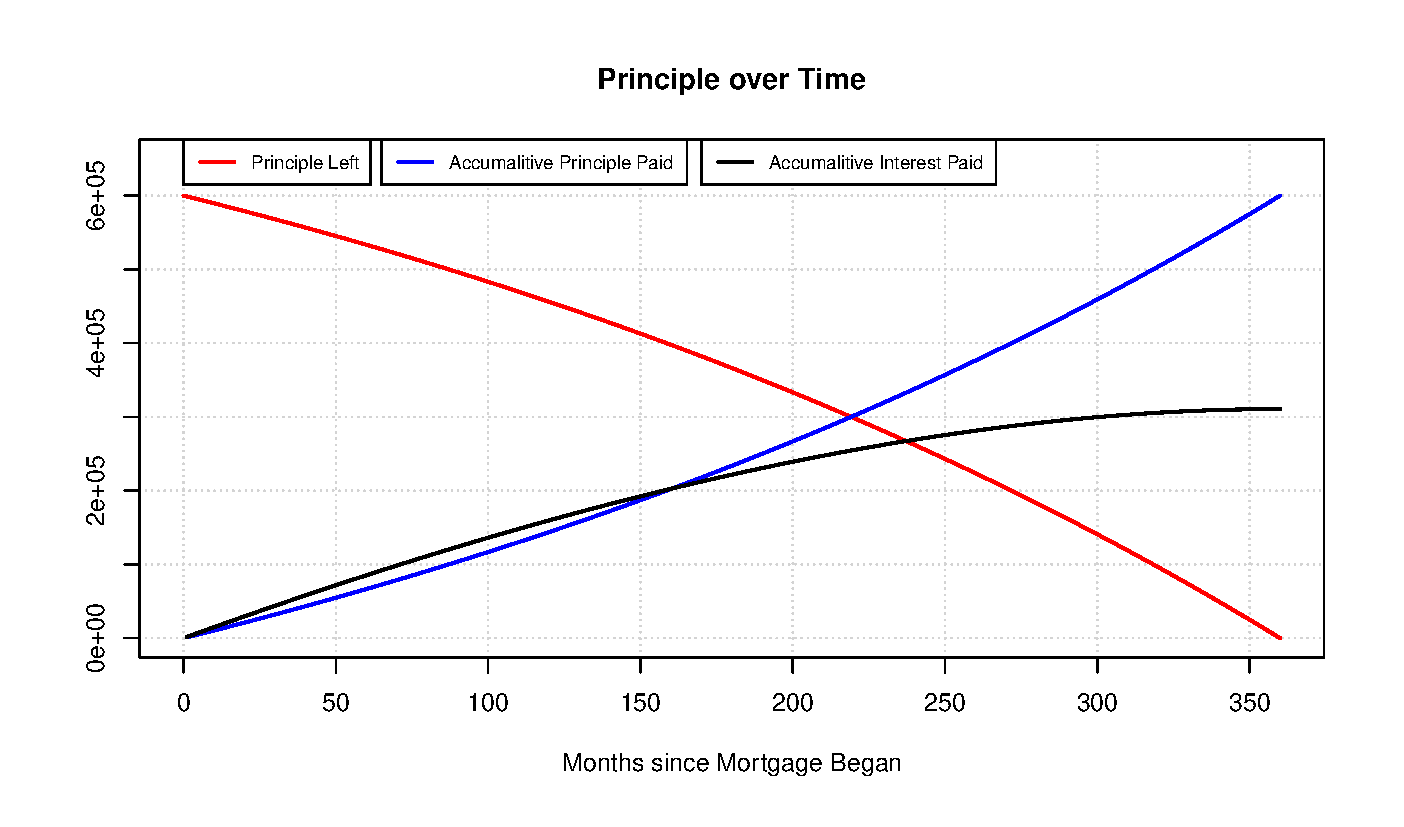
\includegraphics[width = \linewidth, height = 8.4cm]{Figures/POT.C740.S100.T30}
			\includegraphics[width = \linewidth, height = 8.4cm]{Figures/PVT.C740.S100.T30}
		\end{figure}
	\end{Section}

	\begin{Section}{Example B}
		\textbf{\Huge Example B}
		\\ \\
		Let there be a Client B with a credit score 680, an annual salary of \$65,000 and looking for a 30 year term loan.  This client will represent someone who will have the minimum credentials to purchase a home in San Diego.  They will be looking for a home with the minimum home value in San Diego, \$500,000, and because of their credit will unfortunately get the highest interest rate of 3.50\%
		\\  \\
		With a credit score of 680, we can estimate the annual interest rate to be 3.50\% and with the given salary, term length, and interest rate, Client B can be pre-approved for a max loan of \$482,505.80. We can round this to \$482,500.  This will lead to a monthly payment of \$2,166.64, which will make Client B's monthly housing expense take up 40\% of his' or her's monthly income.   If Client B puts down the minimum down payment, 3.5\%, Client B will only be able to afford a \$500,000 home; this is one of the cheaper homes that can be purchased in San Diego.  By the end of the mortgage, Client B will have paid in a total of \$779,990.62 for a \$482,500 loan.  This means, the client would have paid a total of \$297,490.62 worth of interest.  This is 61.66\% the original loan in just interest.  It takes 19 years and 4 months to have paid more principle than interest.  On a month to month aspect, it takes 10 years and 4 months for the monthly payment to pay more principle than interest. 
		\\ \\
		If Client B waits to improve their credit score before buying the home, they can decrease their annual interest rate to 3.00\%.  This will change the total interest paid to \$249,826.21, which will save him or her \$47,664.41.  Another Option would be for Client B to refinance as soon as possible to decrease their interest rate.  This will allow Client B to begin a new loan with lower interest, however, with the downside of repeating the term length.  A good solution to this is to appraise the value of the home, which will make refinancing turn a profit, which will pay for the extra years, and come with a lower interest rate.
		\\
		\begin{figure}[h!]
			\centering
			\includegraphics[width = \linewidth]{Figures/POT.C680.S65.T30}
			\includegraphics[width = \linewidth]{Figures/PVT.C680.S65.T30}
		\end{figure}
	\end{Section}

	\begin{Section}{Example C}
		\textbf{\Huge Example C}
		\\ \\
		Let there be a Client C with a credit score 800, an annual salary of \$130,000 and looking for a 30 year term loan. This client will represent someone who can afford an upper middle class home in San Diego.  They will be looking a very high home value in San Diego, \$1,000,000 and because of their almost perfect credit will receive the lowest interest rate of 2.50\%.
		\\ \\
		With a credit score of 800, we can estimate the annual interest rate to be 2.50\% and with the given salary, term length, and interest rate, Client C can be pre-approved for a max loan of \$822,533.06.  We will round this to \$800,000.  This will lead to a monthly payment of \$3,160.97. If the client puts down a 20\% down payment, Client C will be able to afford a \$1,000,000 home.  By the end of the mortgage, Client C will have paid a total of \$1,137,948.19 for a \$800,000 loan. This means, the client would have paid a total of \$337,948.19 worth of interest.  This is 42.24\% the original loan in just interest.  It takes 5 years and 7 months, to have paid more principle than interest.  On a month to month aspect, it takes 2 years and 4 months for the monthly payment to pay more principle than interest. 
		\\ \\
		If Client C wanted to get a 15 year term, he or she could get approved for a \$480,000 loan.  With a 20\% down payment, they can get a \$600,000 home in San Diego.  This would make their monthly payment only \$3,200.59.  Because of the lower principle, low interest rate, and short term, every monthly payment is paying more of the principle than interest.  They would pay a total of \$576,105.88 on a \$480,000 loan.  This means they would pay \$96,105.88, which is only 20\% of the original loan.       
		\newpage
		\textbf{\Large P: \$800,000, I: 2.5\%, T: 30 Years}
		\begin{figure}[h!]
			\centering
			\includegraphics[width = \linewidth]{Figures/POT.C800.S130.T30}
			\includegraphics[width = \linewidth]{Figures/PVT.C800.S130.T30}
		\end{figure}
		\newpage
		\textbf{\Large P: \$480,000, I: 2.5\%, T: 15 Years}
		\begin{figure}[h!]
			\centering
			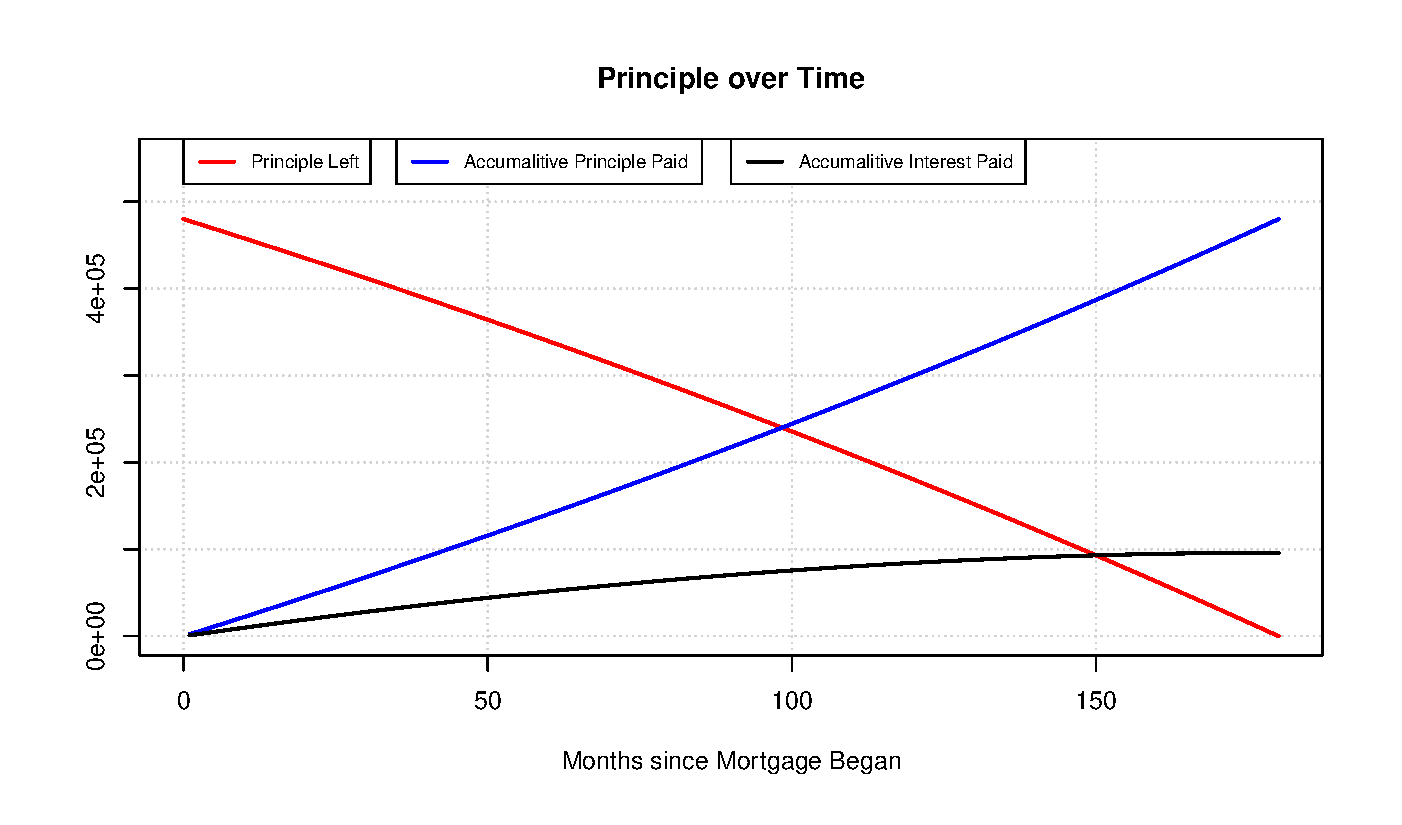
\includegraphics[width = \linewidth]{Figures/POT.C800.S130.T15}
			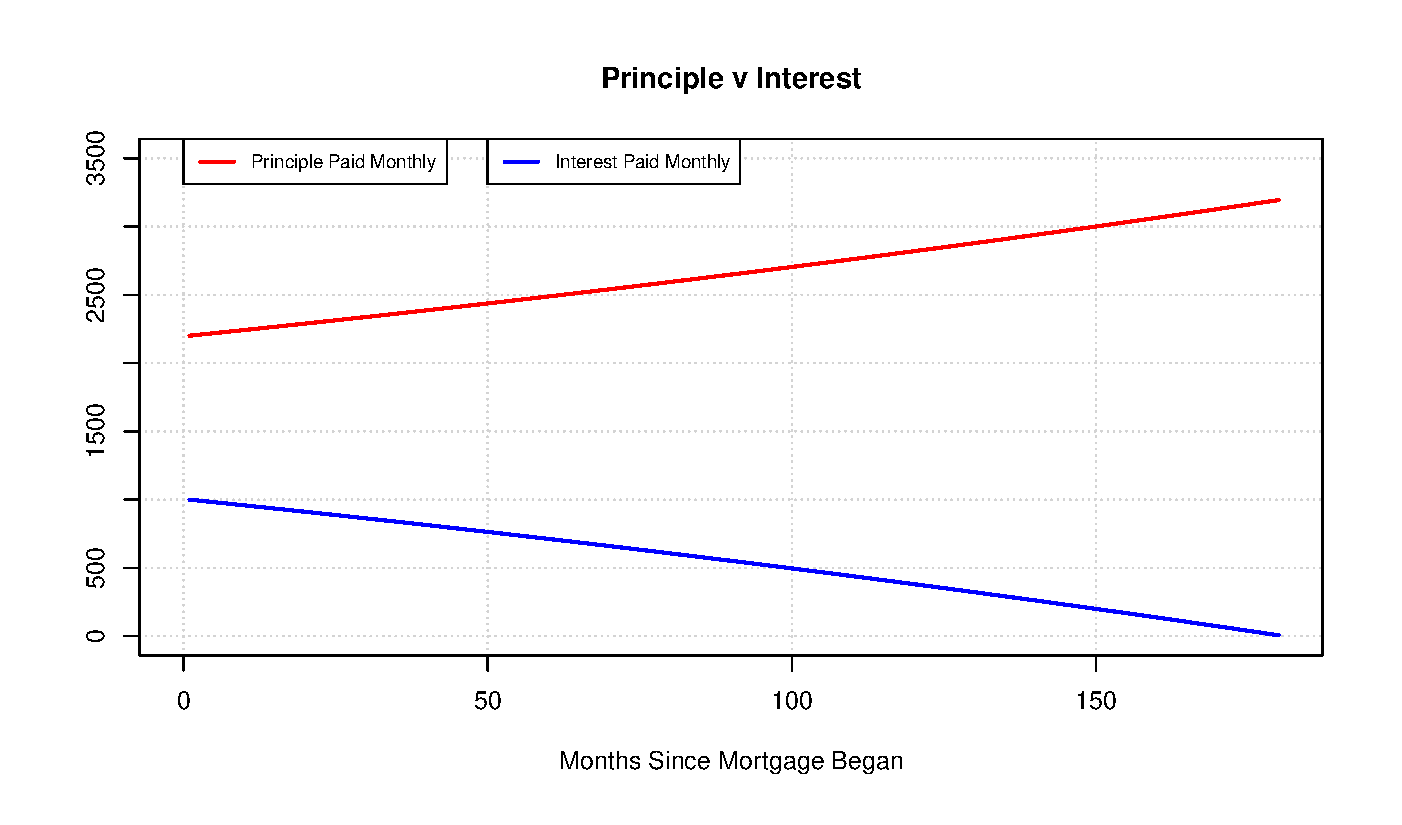
\includegraphics[width = \linewidth]{Figures/PVT.C800.S130.T15}
		\end{figure}
	\end{Section}

	\begin{Section}{Sensitivity}
		\textbf{\Huge Sensitivity Analysis}
		\\ \\
		Please notice and download the following data for different down payments on the following website:
		\\
		\url{https://stepheng753.com/Math336Project/}
		\\ 
		It contains all data on different term lengths, different principals, different interest rates.
		\\ \\
		From this data, we can see how slight variations in interest rates can change monthly payments and amount of interest accrued through the lifetime of the mortgage.  Notice a simple 4.1667\% change in interest rate can change the amount of interest accrued by about 4.70\%.  This is important because many clients wont see the harm in choosing an interest rate of 2.875\% versus a 3.00\%.  That 4\% change in interest rate will be the difference of up to \$20,000 in the long term.  Clients can also be blindsided in the fact that the 4\% change in interest rate will lead to only a 0.8-1.6\% change in their monthly payment.  However, it is in the best interest for the customer to understand the long term affects more than the short term affects.  
	\end{Section}

	\begin{Section}{Conclusions}
		\textbf{\Huge Conclusions}
		\\ \\
		Looking at the 3 examples, we are able to examine the following:
		\\ \\
		The most important things to consider when trying to buy a home is your credit score, your income, and the amount you are able to put down for a down payment.  All these things greatly affect your mortgage loan.  
		\\ \\
		In Example A and B, we were able to see how much money each client could save with better credit scores, which would lead to a better interest rate.  We were also able to see that different income levels led to each getting drastically different houses and down payments.  Notice how Client A was paying only \$363 more a month than Client B for a \$250,000 richer house.  This is because Client A was purchasing a house about worth the same as Client B in relation to their income.  We could easily see that if Client A got the same loan with his interest rate of 3\% and 20\% down payment, the monthly payment would be a lot smaller. It would be \$480 less than Client B's monthly payment for the same amount borrowed. 
		\\ \\ 
		From Example C, we were able to see that with the highest credit score, a very high income, the interest can be very minimized.  Client C was shown to pay the least amount of interest in relation to the original loan given.  Client C also shows us the affect in term length.  Term length greatly changes the amount a Client needs to pay in interest.  With a shorter term length, each monthly payment is more focused on paying off the principle than the interest, which will thus lead to a significant decrease in overall interest than with a longer term length. 
	\end{Section}
	
	\begin{Section}{Bibliography}
		\textbf{\Huge Bibliography}
		\\ \\ \\
		\url{https://www.nerdwallet.com/mortgages/mortgage-rates/california/san-diego}
		\\ \\
		\url{https://www.experian.com/blogs/ask-experian/what-credit-score-do-i-need-to-buy-a-house/}
		\\ \\
		\url{https://www.youtube.com/watch?v=zOHJUVSAeDw&t=90s&ab_channel=TwoCents}
		\\ \\
		\url{https://www.payscale.com/cost-of-living-calculator/California-San-Diego}
		\\ \\
		\url{https://www.zillow.com/san-diego-county-ca/home-values/#:~:text=%24632%2C264&text=The%20typical%20home%20value%20of,7.5%25%20in%20the%20next%20year.}
	\end{Section}


\end{document}
